\documentclass{beamer}

\usepackage{comment}
\usepackage{color}
\usepackage{listings}
\usepackage{verbatim}
\usepackage{multicol}
\usepackage{booktabs}
\definecolor{green}{RGB}{0,128,0}

\def\EQ#1\EN{\begin{equation*}#1\end{equation*}}
\def\BA#1\EA{\begin{align*}#1\end{align*}}
\def\BS#1\ES{\begin{split*}#1\end{split*}}
\newcommand{\bc}{\begin{center}}
	\newcommand{\ec}{\end{center}}
\newcommand{\eq}{\ =\ }
\newcommand{\degc}{$^\circ$C}

\def\p{\partial}
\def\qbs{\boldsymbol{q}}
\def\Dbs{\boldsymbol{D}}
\def\A{\mathcal A}
\def\gC{\mathcal C}
\def\gD{\mathcal D}
\def\gL{\mathcal L}
\def\M{\mathcal M}
\def\P{\mathcal P}
\def\Q{\mathcal Q}
\def\gR{\mathcal R}
\def\gS{\mathcal S}
\def\X{\mathcal X}
\def\bnabla{\boldsymbol{\nabla}}
\def\bnu{\boldsymbol{\nu}}
\renewcommand{\a}{{\alpha}}
%\renewcommand{\a}{{}}
\newcommand{\s}{{\sigma}}
\newcommand{\bq}{\boldsymbol{q}}
\newcommand{\bz}{\boldsymbol{z}}
\def\bPsi{\boldsymbol{\Psi}}

\def\Li{\textit{L}}
\def\Fb{\textbf{f}}
\def\Jb{\textbf{J}}
\def\cb{\textbf{c}}

\def\Dt{\Delta t}
\def\tpdt{{t + \Delta t}}
\def\bpsi{\boldsymbol{\psi}}
\def\dbpsi{\delta \boldsymbol{\psi}}
\def\bc{\textbf{c}}
\def\dbc{\delta \textbf{c}}
\def\arrows{\rightleftharpoons}

\newcommand{\bGamma}{\boldsymbol{\Gamma}}
\newcommand{\bOmega}{\boldsymbol{\Omega}}
%\newcommand{\bPsi}{\boldsymbol{\Psi}}
%\newcommand{\bpsi}{\boldsymbol{\psi}}
\newcommand{\bO}{\boldsymbol{O}}
%\newcommand{\bnu}{\boldsymbol{\nu}}
\newcommand{\bdS}{\boldsymbol{dS}}
\newcommand{\bg}{\boldsymbol{g}}
\newcommand{\bk}{\boldsymbol{k}}
%\newcommand{\bq}{\boldsymbol{q}}
\newcommand{\br}{\boldsymbol{r}}
\newcommand{\bR}{\boldsymbol{R}}
\newcommand{\bS}{\boldsymbol{S}}
\newcommand{\bu}{\boldsymbol{u}}
\newcommand{\bv}{\boldsymbol{v}}
%\newcommand{\bz}{\boldsymbol{z}}
\newcommand{\pressure}{P}

\def\water{H$_2$O}
\def\calcium{Ca$^{2+}$}
\def\copper{Cu$^{2+}$}
\def\magnesium{Mg$^{2+}$}
\def\sodium{Na$^+$}
\def\potassium{K$^+$}
\def\uranium{UO$_2^{2+}$}
\def\hion{H$^+$}
\def\hydroxide{0H$^-$}
\def\bicarbonate{HCO$_3^-$}
\def\carbonate{CO$_3^{2-}$}
\def\cotwo{CO$_2$(aq)}
\def\chloride{Cl$^-$}
\def\fluoride{F$^-$}
\def\phosphoricacid{HPO$_4^{2-}$}
\def\nitrate{NO$_3^-$}
\def\sulfate{SO$_4^{2-}$}
\def\souotwooh{$>$SOUO$_2$OH}
\def\sohuotwocothree{$>$SOHUO$_2$CO$_3$}
\def\soh{$>$SOH}

\newcommand\gehcomment[1]{{{\color{orange} #1}}}
\newcommand\add[1]{{{\color{blue} #1}}}
\newcommand\remove[1]{\sout{{\color{red} #1}}}
\newcommand\codecomment[1]{{{\color{green} #1}}}
\newcommand\redcomment[1]{{{\color{red} #1}}}
\newcommand\bluecomment[1]{{{\color{blue} #1}}}
\newcommand\greencomment[1]{{{\color{green} #1}}}
\newcommand\magentacomment[1]{{{\color{magenta} #1}}}

\begin{comment}
\tiny
\scriptsize
\footnotesize
\small
\normalsize
\large
\Large
\LARGE
\huge
\Huge
\end{comment}

\begin{document}
\title{Capstone Problem}
%\author{Ethan Conley}
\date{\today}

%\frame{\titlepage}

\section{Location of Example}

\begin{frame}[fragile,containsverbatim]\frametitle{Location}

Location of the crystalline capstone problem:

\begin{semiverbatim}
> cd \$PFLOTRAN_DIR
> cd shortcourse/exercises/crystalline_capstone
> ls

run_sampling.in    \bluecomment{! dakota input file }
samples            \bluecomment{! directory containing dakota 
                     samples \& results}
dakota_driver      \bluecomment{! directory containing supporting
                     files called in run_sampling.in}
dfn_generation     \bluecomment{! directory containing files to
                     generate the fracture network}
clean_up_dakota.sh \bluecomment{! executable to clean directories 
                     for restart }
doc                \bluecomment{! directory containing documentation
                     for capstone problem}
\end{semiverbatim}

\end{frame}

%-----------------------------------------------------------------------------
\section{Description of Crystalline Capstone Problem}

\subsection{Crystalline Capstone Conceptual Model}

\begin{frame}\frametitle{Description of Crystalline Capstone Scenario}
Challenge yourself by setting up an input deck to simulate the ``\gehcomment{Crystalline Capstone Scenario}.'' It features:
\begin{itemize}
  \item Problem domain: $1000 \times 1000 \times 500$ m (x $\times$ y $\times$ z)
  \item Grid resolution: $50 \times 100 \times 20$ m (x $\times$ y $\times$ z) (\redcomment{Structured grid})
  \item SUBSURFACE\_FLOW MODE \redcomment{RICHARDS}
  \item \redcomment{Hydrostatic} initial conditions
  \item Recharge (\redcomment{Neumann} boundary condition)
  \item Radionuclide Sources: Defined with \redcomment{WASTE\_FORM}
  \item Radionuclide Behavior: Controlled with \redcomment{UFD\_DECAY}
  \item Injection of four tracers into repository region
  \item Leak from waste package (represents breach of waste package)
  \item Aqueous, solid, sorbed phases, radioactive decay
  \item Total simulation time: 1,000,000 y
\end{itemize}

\end{frame}

%-----------------------------------------------------------------------------
\begin{frame}{\frametitle{Crystalline Capstone Scenario Schematic}
\begin{center}
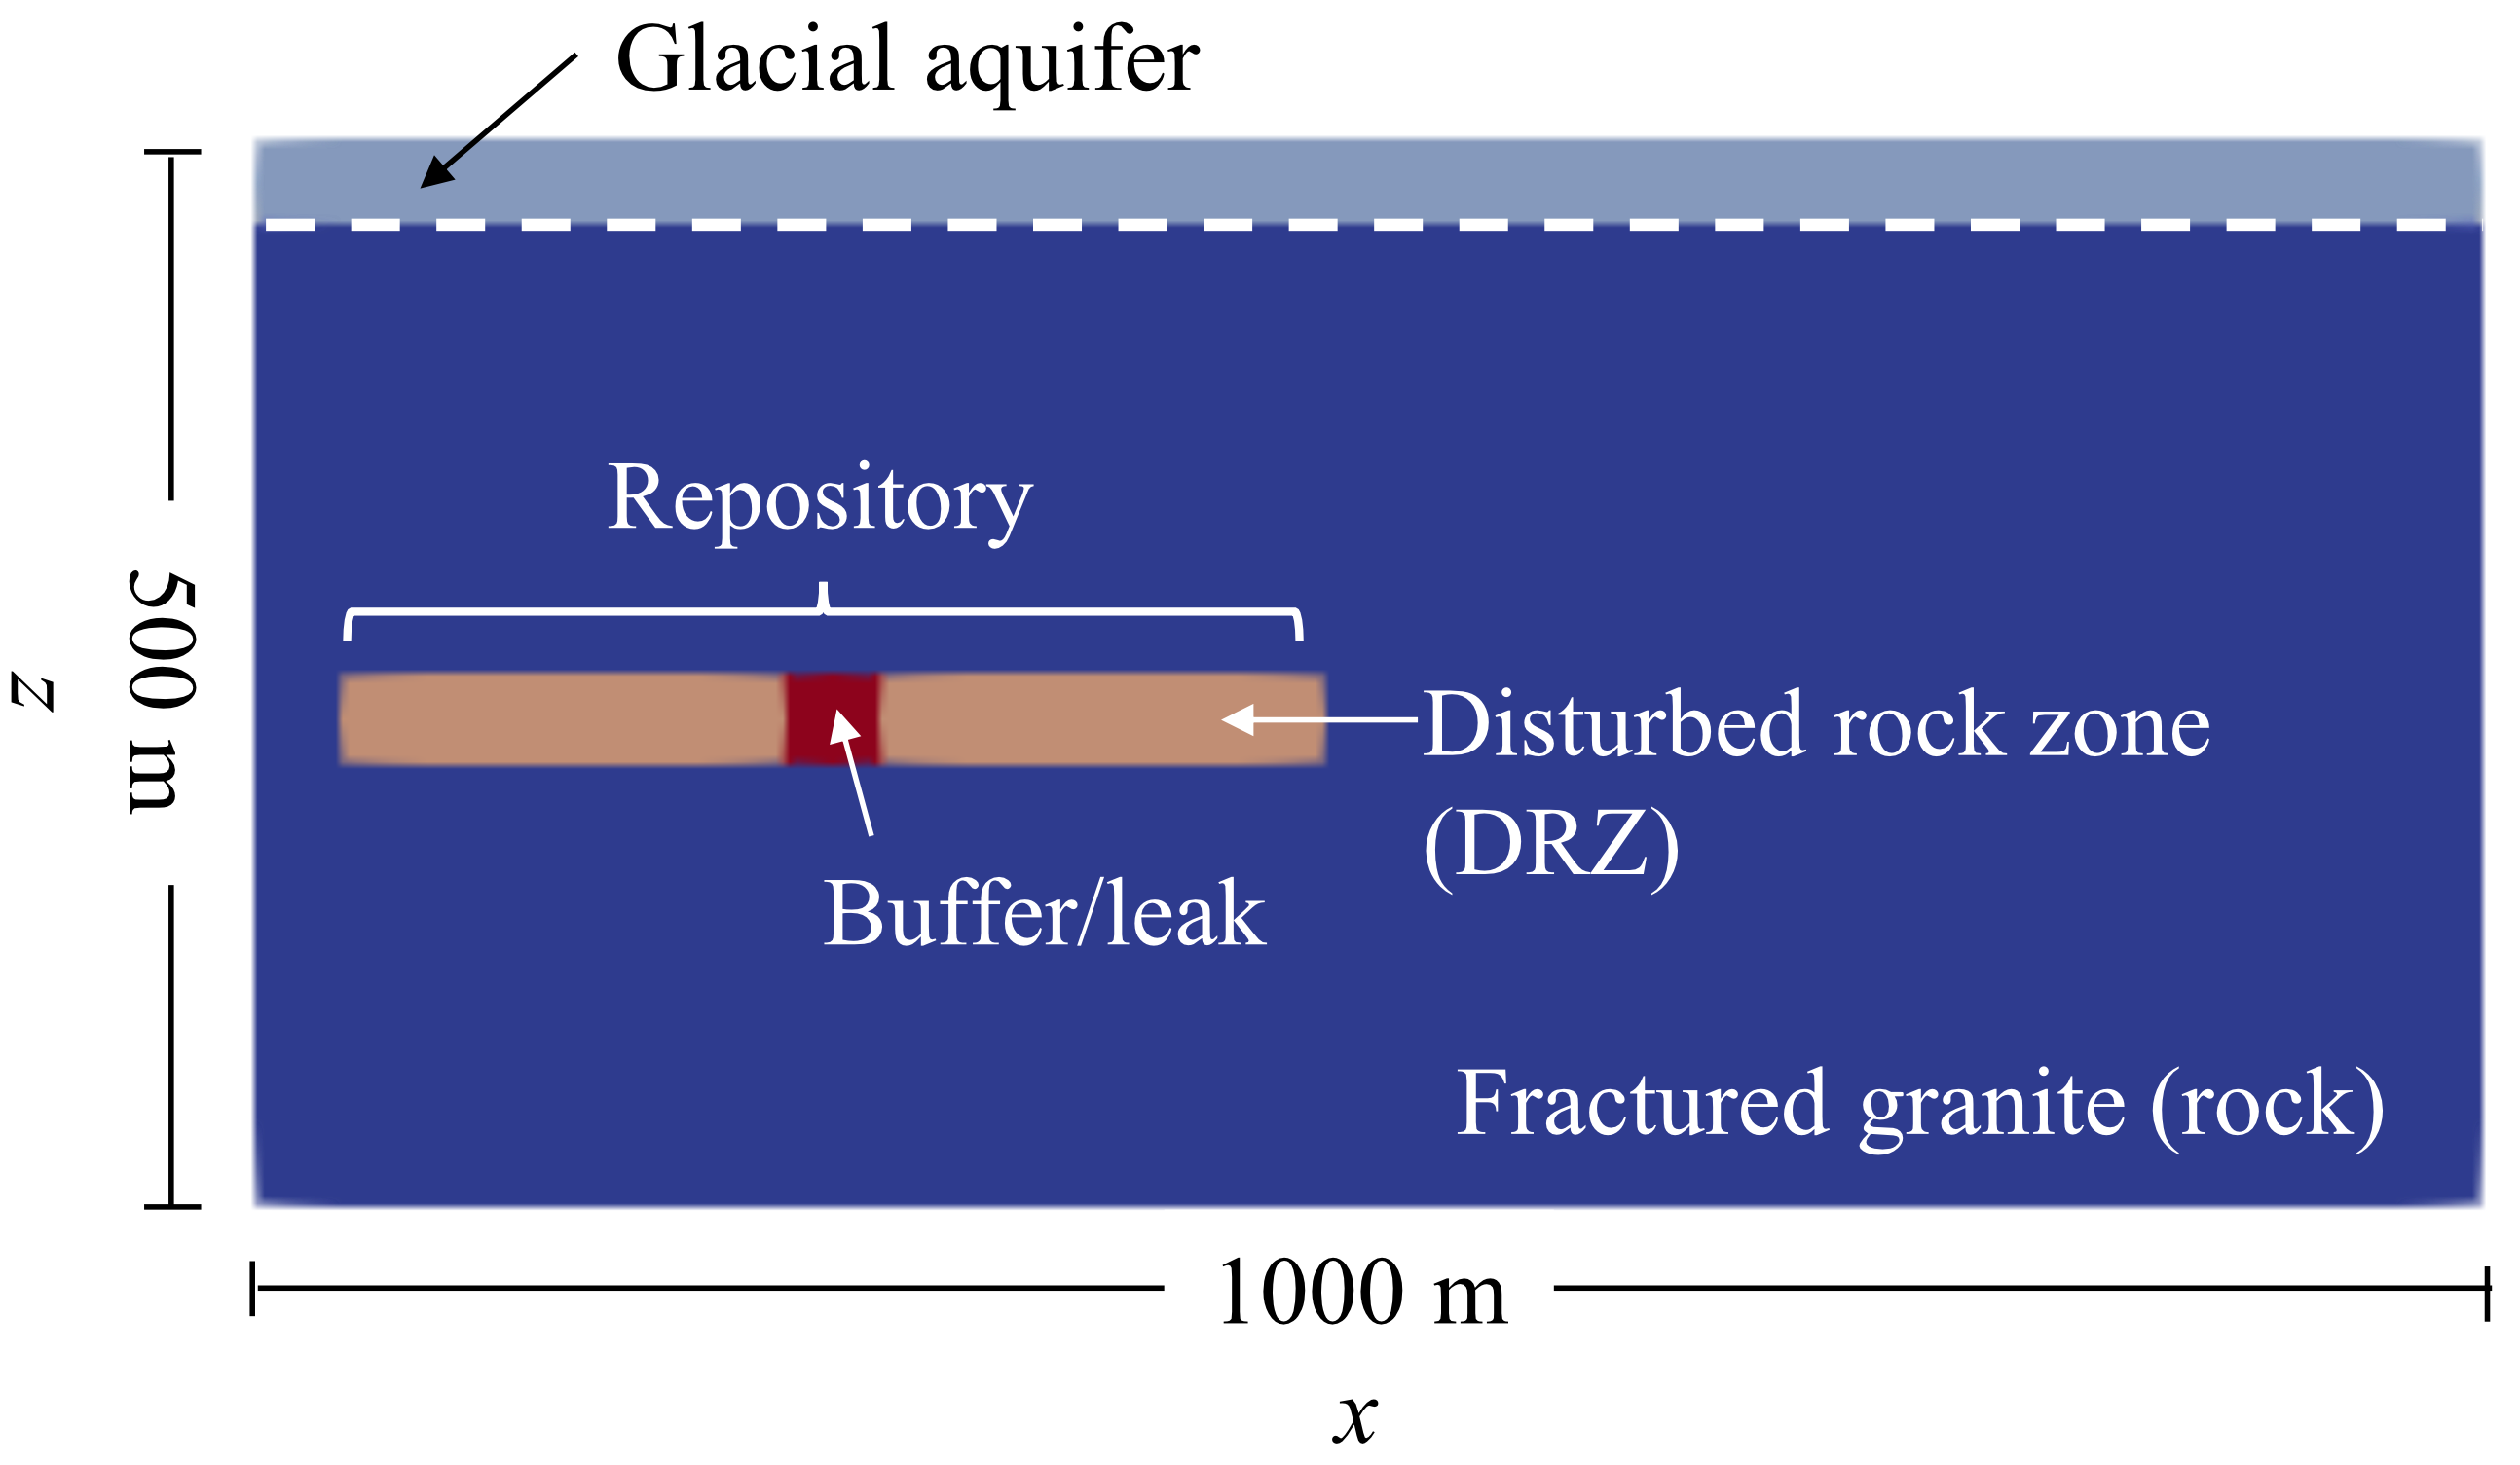
\includegraphics[width=12cm]{./domain_diagram.png}
\end{center}
}
\end{frame}

%-----------------------------------------------------------------------------
\begin{frame}\frametitle{Setup}
	Here's some information on the setup of the PFLOTRAN input deck:
	\begin{itemize}
		\item The repository is located at: [40-480 m, 280-720 m, 200-240 m]
		\item The waste package (leak) is located at: [240-280 m, 480-520 m, 200-240 m]. The "buffer" material can be applied to the waste package area.
		\item The glacial aquifer is located at: [0-1000 m, 0-1000 m, 440-500 m]
		\item Initial Condition: Hydrostatic pressure with a head gradient of -0.0013m/m from left to right with pressure of 101325 Pa at a datum of [1000, 0, 500] (top right)
		\item A Source term (inject\_repos) injecting water with tracer at 3.17x10$^{-14}$ m$^3$/s, scaled by volume (RATE SCALED\_VOLUMETRIC\_RATE VOLUME) 
		\item Boundary Conditions: 2 mm/yr infiltration rate along the top boundary with initial transport conditions, initial conditions along the west and east boundaries.
	\end{itemize}
	
\end{frame}

\begin{frame}\frametitle{Setup}
		\begin{itemize}
			\item Initial concentrations everywhere of all species equal to 1x10${^-22}$ M, except Tracer1 concentration is initially 1x10$^{-1}$ M in the repository area (init\_repos)
			\item Injection concentrations of Tracers 2, 3, and 4 of 1x10$^{-2}$ M in the injection area (inject\_repos)
			\item I-129: Solubility = 1x10$^4$ M (infinitely soluble), kd = 0 everywhere (non-sorbing), and Decay Rate = 1.29x10$^{-15}$/s
			\item Tracer 1: non-decaying, non-sorbing, pulses by setting a non-zero concentration as an initial condition and background concentration after.
			\item Tracer 2: non-decaying, non-sorbing, infinitely soluble, injected with the source term
			\item Tracer 3: decays at a decay rate of 2.2x10$^{-13}$ /s, infinitely soluble, injected with the source term
			\item Tracer 4: non-decaying, sorbs with kd's: [buffer : 1.76x10$^8$; granite : 1.73x10$^7$; drz : 1.73x10$^7$; glacial : 6.43x10$^6$], infinitely soluble, injected with the source term
		\end{itemize}
			
\end{frame}


\subsection{The Problem}

\begin{frame}[fragile]\frametitle{The Problem}
	A leak in the waste package occurs some time after repository closure. The biggest concern is the peak $^{129}$I concentration that makes it to the aquifer from the breached waste package. Additionally, we will inject several other tracers from the repository, to examine their release to the aquifer over time.
	\begin{itemize}
		\item \textbf{$^{129}$I}: $^{129}$I is released when the waste package breaches.
		\item \textbf{Tracer Test 1}: A stable conservative tracer is injected into the repository region at the beginning of the simulation.
		\item \textbf{Tracer Test 2}: Identical concentrations of three conservative tracers are continuously injected at a constant rate into the repository. One tracer decays exponentially, one tracer sorbs, and the other tracer remains stable.
	\end{itemize}
	\textbf{Main Goal}: Perform a sensitivity analysis to determine which of the uncertain parameters exerts the most control on $^{129}$I transport.
\end{frame}

%-----------------------------------------------------------------------------
\subsection{Fractures}

\begin{frame}[fragile,containsverbatim,allowframebreaks]\frametitle{Fractures}
	
	The crystalline host rock contains 2 deterministic fractures and 3 families of stochastic fracture networks. The properties are:
	
	Stochastic Fracture Properties
	\begin{itemize}
		\item Fracture Family 1
		\begin{itemize}
			\item Shape: ellipse
			\item Distribution: Truncated Power Law (TPL)
			\item Fracture Intensity (p32): 0.00769494
			\item von Mises-Fisher Distribution concentration (kappa): 22
			\item TPL alpha: 2.5
			\item Min fracture radius: 30 m
			\item Max fracture radius: 500 m
			\item theta: 90 deg
			\item phi: 0
			\item Beta distribution: 1
			\item Semi-correlated hydraulic permeability:
			\begin{itemize}
				\item alpha: 1x10$^{-13}$
				\item beta: 0.9
				\item sigma: 1.0
			\end{itemize}
		\end{itemize}
	\end{itemize}
\end{frame}
	
\begin{frame}[fragile,containsverbatim,allowframebreaks]\frametitle{Fractures}
	\begin{itemize}
		\item Fracture Family 2
		\begin{itemize}
			\item Shape: ellipse
			\item Distribution: Truncated Power Law (TPL)
			\item Fracture Intensity (p32): 0.0055714
			\item von Mises-Fisher Distribution concentration (kappa): 22
			\item TPL alpha: 2.7
			\item Min fracture radius: 30 m
			\item Max fracture radius: 500 m
			\item theta: 180 deg
			\item phi: 90 deg
			\item Beta distribution: 1
			\item Semi-correlated hydraulic permeability:
			\begin{itemize}
				\item alpha: 1x10$^{-13}$
				\item beta: 0.9
				\item sigma: 1.0
			\end{itemize}
		\end{itemize}
	\end{itemize}
	
\end{frame}	
	
	
\begin{frame}[fragile,containsverbatim,allowframebreaks]\frametitle{Fractures}
	\begin{itemize}
		\item Fracture Family 3
		\begin{itemize}
			\item Shape: ellipse
			\item Distribution: Truncated Power Law (TPL)
			\item Fracture Intensity (p32): 0.03376919
			\item von Mises-Fisher Distribution concentration (kappa): 10
			\item TPL alpha: 2.7
			\item Min fracture radius: 30 m
			\item Max fracture radius: 500 m
			\item theta: 0 deg
			\item phi: 360 deg
			\item Beta distribution: 1
			\item Semi-correlated hydraulic permeability:
			\begin{itemize}
				\item alpha: 1x10$^{-13}$
				\item beta: 0.9
				\item sigma: 1.0
			\end{itemize}
		\end{itemize}
	\end{itemize}

\end{frame}
	
\begin{frame}[fragile,containsverbatim,allowframebreaks]\frametitle{Fractures}
	Deterministic Fracture Properties
	\begin{itemize}
		\footnotesize
		\item Fracture 1
		\begin{itemize}
			\item Radius: 200 m
			\item Translation: [500, 500, 250]
                        \item Beta: 0
                        \item Aspect Ratio: 1
			\item Normal Vector: [0,0,1]
			\item Aperture: $\eq 1x10^{-3}$ m
		\end{itemize}
		\item Fracture 2
		\begin{itemize}
			\item Radius: 1000 m
			\item Translation: [-200, -350, 200]
                        \item Beta: 0
                        \item Aspect Ratio: 1
			\item Normal Vector: [1,1,-1]
			\item Aperture: $\eq 4x10^{-3}$ m
		\end{itemize}
	\end{itemize}
	
\end{frame}


%-----------------------------------------------------------------------------
\subsection{Uncertainty}

\begin{frame}[fragile]\frametitle{Uncertain Parameters}

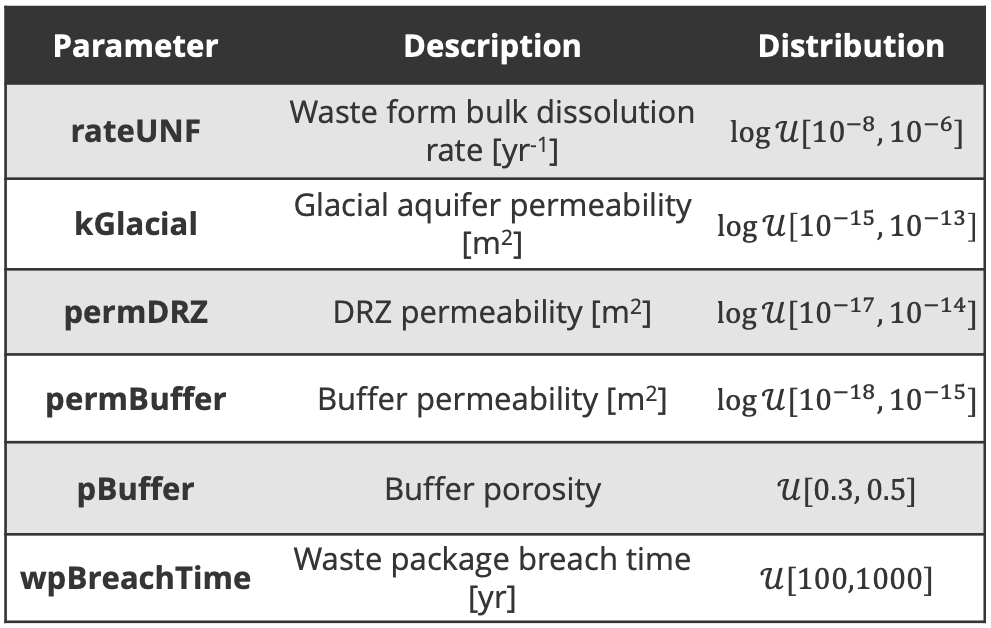
\includegraphics[width=\linewidth]{dakota_params.png}
\end{frame}

%-----------------------------------------------------------------------------
\subsection{Samples}

\begin{frame}[fragile]\frametitle{Sampling on Uncertain Parameters}
In the Dakota input file, there is an option for how many samples of each parameter you'd like to include in your analysis. \\
Consider how many realizations you need to sufficiently reduce uncertainty and capture the sensitivity of each parameter. \\
Start with 10 samples, and go from there. Choose your sampling method (e.g., random, Latin Hypercube). \\
\begin{itemize}
    \item This should be the number of samples specified in the Dakota input file \\
\end{itemize}
Results of each model realization will be located in "samples" directory \\
\begin{itemize}
    \item Each iteration's results located in respective folders workdir.1, workdir.2, ..., workdir.n
\end{itemize}

\end{frame}

%-----------------------------------------------------------------------------
\subsection{Add Observation Points}

\begin{frame}[fragile]{Add Observation Points}
Add observation point in repository to observe concentrations of tracer 1 and an additional observation point in downstream portion of glacial aquifer to observe concentrations of tracers 2, 3, \& 4 \\
\textbf{   }\\
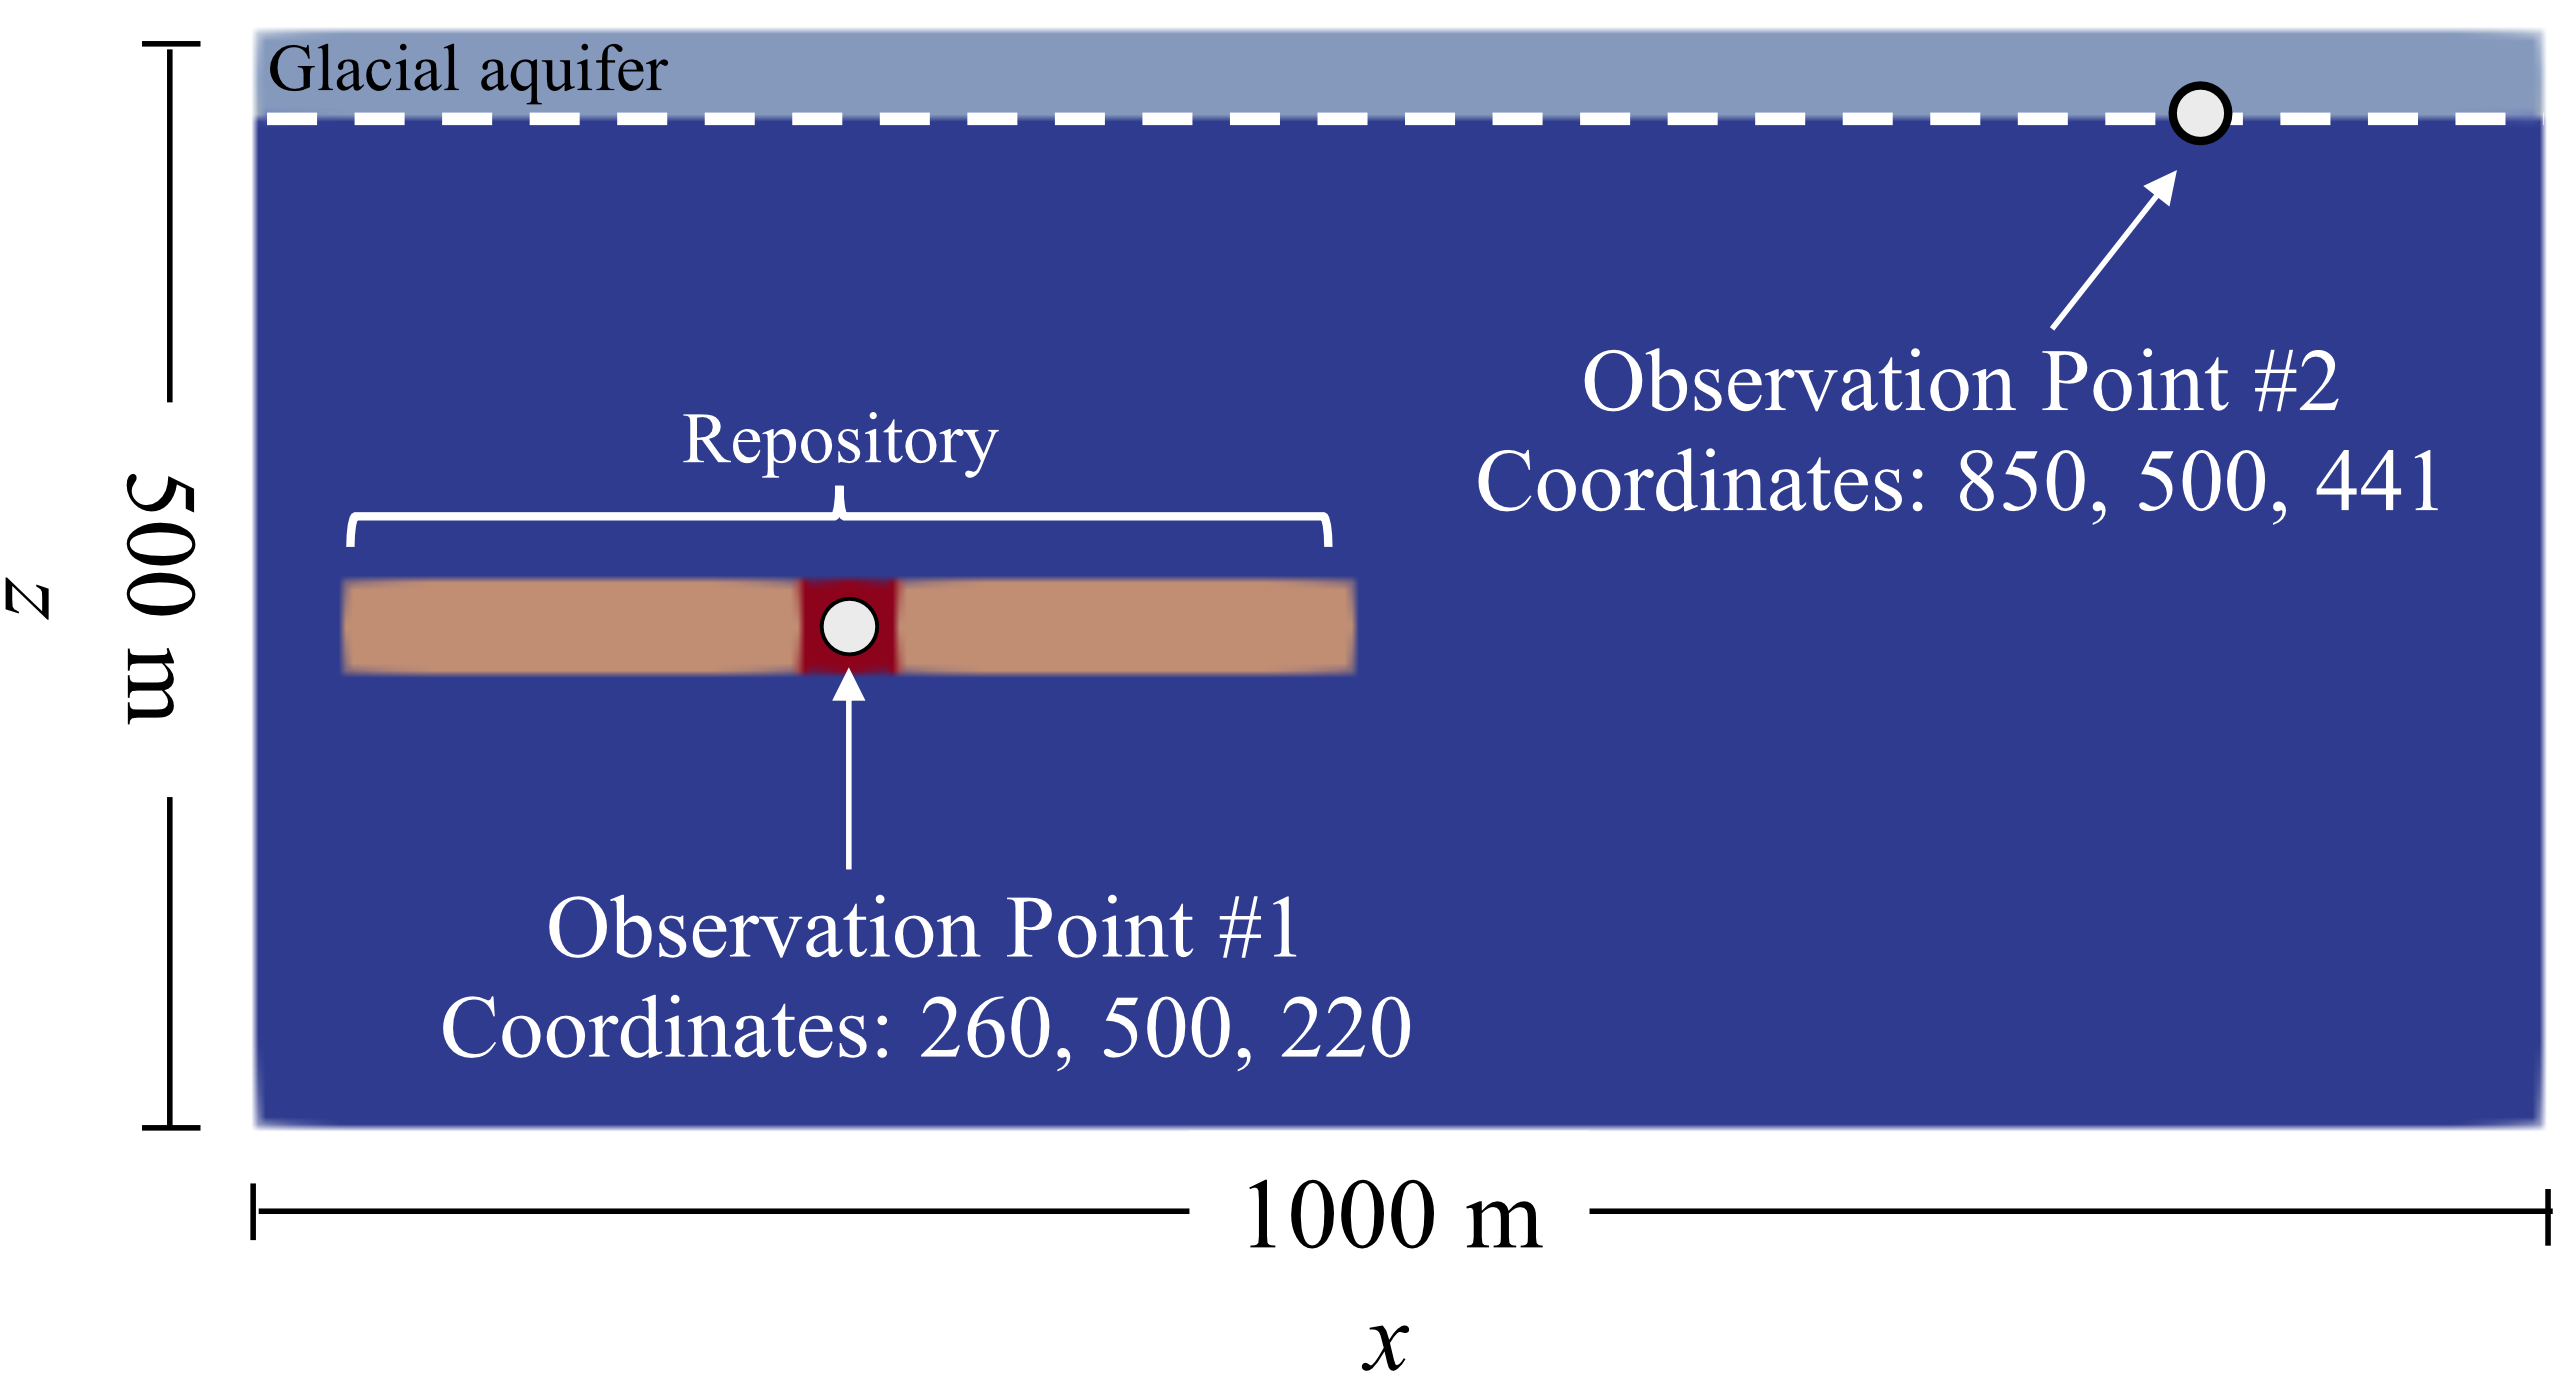
\includegraphics[width=\linewidth]{./observation_point.png}

\end{frame}

%-----------------------------------------------------------------------------
\subsection{Template}

\begin{frame}[fragile]{Templates}	
       \begin{itemize}
    		\item We have included a skeleton of create\_dfn.py for adding in fracture network properties which should be ran before PFLOTRAN.
		\item We have included a skeleton of the pflotran.template file that Dakota will use. You will modify this once you have your PFLOTRAN model ready to run.
		\item We have included a skeleton of the run\_sampling.in file for Dakota. 
		\item \textbf{Look for "..." in each of these files. These indicate that something is missing from the file here.}
		\item Use the directory "workspace" to test run your PFLOTRAN simulations. You will ultimately use the pflotran.in file you build here to put together the pflotran.template file in the "dakota\_driver" directory.
		\item The Python script "plot\_results.py" has been provided for you. This will plot concentrations vs time at observation points and collect information from Dakota output. Modify this to fit your particular model and plotting needs.
	\end{itemize}
	
\end{frame}

%-----------------------------------------------------------------------------
\subsection{Steps to Create Input Files}

\begin{frame}[fragile]{Steps to Create Input Files}
  
\begin{enumerate}
  \item Create fracture network and upscale to an ECPM.
  \begin{enumerate}
    \item We have included a skeleton of create\_dfn.py in the directory  "dfn\_generation". You will add in the fracture network properties to this file. \textbf{This should be completed and ran before moving on to editing the PFLOTRAN input file and running Dakota.}
    \item When create\_dfn.py is ready, in the dfn\_generation folder run: ./run\_dfn.sh (this will create the fracture network and upscale)
  \end{enumerate}
  \item Build the pflotran.template file.
  \begin{enumerate}
    \item  Use the directory "workspace" to test run your PFLOTRAN simulations without Dakota. You will ultimately use the pflotran.in file you build here to put together the pflotran.template file in the "dakota\_driver" directory.
    \item  We have included a skeleton of the pflotran.template file that Dakota will use in "dakota\_driver". You will modify this once you have your PFLOTRAN model ready to run.
  \end{enumerate}
  \item Build the Dakota input file: We have included a skeleton of the run\_sampling.in file for Dakota.
\end{enumerate}


\end{frame}

%-----------------------------------------------------------------------------

\subsection{Running the Problem}

\begin{frame}[fragile]{Running the Problem}
	
	\begin{itemize}
                \item When you have everything ready to go and the fractures are generated, cd to the top-level crystalline-capstone directory.
                \item To begin, make sure that the run directory is clean: ./clean\_up\_dakota.sh
		\item Then, run: dakota run\_sampling.in
                \begin{itemize}
                  \item The results for each iteration can be found in the samples directory.
                \end{itemize}
		\item You can plot results using the provided Python script plot\_results.py
                \begin{itemize}
                  \item This will plot concentrations vs time at observation points and collect information from Dakota output. Modify this to fit your particular model and plotting needs.
                \end{itemize}
		\item Use plots and analysis of the Dakota output to answer the following questions:
	\end{itemize}
	
\end{frame}

%-----------------------------------------------------------------------------


\subsection{Challenge Problems}

\begin{frame}[fragile]\frametitle{Challenge Problem Question \#1}
	\textbf{$^{129}$I:} Show the concentration of $^{129}$I as a function of time at both the repository observation point and the aquifer observation point for all model realizations.  \\
	\textbf{    }\\
	\textbf{Question 1a: }\textit{Which of the uncertain parameters exerts the most control on max $^{129}$I concentration in the aquifer?}
	\textbf{    }\\
	\textbf{Question 1b: }\textit{What is the probability that the max $^{129}$I concentration in the aquifer will be below 1x10$^{-16}$ M?}
\end{frame}

%-----------------------------------------------------------------------------
\subsection{Challenge Problems}

\begin{frame}[fragile]\frametitle{Challenge Problem Question \#2}
	
	\textbf{Tracers:} Show the concentration of all tracers as a function of time at the observation point located in the downstream portion of the glacial aquifer for all model realizations.  \\
	\textbf{    }\\
	\textbf{Question 2: }\textit{What is the expected maximum concentration of each tracer in the aquifer at the observation point?}
	
\end{frame}

%-----------------------------------------------------------------------------
\subsection{Challenge Problems}

\begin{frame}[fragile]\frametitle{Challenge Problem Question \#3}
	\textbf{New Information:} You have some new information. The waste package breach time follows a normal distribution with mean = 9,000 years and standard deviation = 1,000 years. You also have discovered a new elliptical fracture with radius 500 m, translation of [-200,-350,200], normal vector [1,1,1], and aperture 2E-03.  \\
	\textbf{    }\\
	\textbf{Question 3b: }\textit{How does your analysis for the above questions change when incorporating this new information?}
	\textbf{    }\\
	\textbf{Question 3b: }\textit{How does your analysis for the above questions change if you increase the number of model realizations?}
\end{frame}

%-----------------------------------------------------------------------------
\subsection{Challenge Problems}

\begin{frame}[fragile]\frametitle{Bonus Questions}
	\textbf{Fracture Uncertainty:} If you were uncertain about the fracture distributions in this problem, how would you incorporate this into your sensitivity analysis? Answer the above questions but also considering uncertainty in fracture properties. \\
	\textbf{Grid Resolution:} What happens if you run the same models on a finer grid? \\
\end{frame}

%-----------------------------------------------------------------------------
\begin{frame}[fragile]\frametitle{If You Get Stuck}
\textbf{Your first step should be to look back at previous short course example input files.}\\
\textbf{   }\\
A complete Dakota input file is located in run\_sampling.in.answers
\begin{itemize}
    \item only use this if you are stuck on a certain portion of the input file
    \item the number of samples in this file is only an example - not necessarily the amount of samples that you should use for your analysis
\end{itemize}
A PFLOTRAN input deck containing answers is located in dakota\_driver/pflotran.template.answers
\begin{itemize}
  \item only use this if you are stuck on a certain section of the input deck
  \item Refer to the documentation at \textit{documentation.pflotran.org} or previous short course problem input decks for assistance with creating observation points, regions, grids, etc. 
\end{itemize} 
A DFN generation script containing answers is located in dfn\_generation/create\_dfn.py.answers
\begin{itemize}
	\item only use this if you are stuck on defining DFN properties for the model.
\end{itemize} 
\end{frame}
%-----------------------------------------------------------------------------
\end{document}
